\frame
{ \frametitle{What is DDL?}

\begin{itemize}
\item ``Data Definition Language''
\item Stuff most people are familiar with
\item<2-> on this room anyway
\begin{itemize}
\item \texttt{CREATE \{ TABLE , FUNCTION , VIEW , ... \} }
\begin{itemize} \item 36 CREATE commands \end{itemize}
\item \texttt{ALTER \{ TABLE, OPERATOR FAMILY, ... \} }
\begin{itemize} \item 37 ALTER commands \item  43 sub-commands ALTER TABLE \end{itemize}
\item \texttt{DROP \{ TABLE, EXTENSION, POLICY, ... \} }
\begin{itemize} \item 36 DROP commands \end{itemize}
\end{itemize}
\end{itemize}
}

\frame
{ \frametitle{How can you capture DDL?}

\begin{itemize}
\item  Use event triggers!
\item  ... which are a relatively new PostgreSQL feature
\begin{itemize} \item introduced in 9.3 \end{itemize}
\item  runs a user-defined function when a database event occurs
\end{itemize}

\vfill

\begin{columns}
\color{gray}
\begin{column}{0.3\textwidth}
\end{column}
\begin{column}{0.7\textwidth}
\raggedleft \footnotesize
The research leading to these results has received funding from the European Union's \href{http://ec.europa.eu/research/fp7/index_en.cfm}{\underline{Seventh Framework Programme (FP7/2007-2013)}} under grant agreement n° 318633
\end{column}
\end{columns}


}

\begin{frame}[fragile]
\frametitle{Syntax of CREATE EVENT TRIGGER}

\begin{lstlisting}
CREATE EVENT TRIGGER name
  ON event
  [ WHEN filter_variable IN (filter_value [, ... ])
       [ AND ... ] ]
  EXECUTE PROCEDURE function_name()
\end{lstlisting}

\end{frame}

\frame
{ \frametitle{What events can occur?}

\begin{itemize}
 \item \texttt{ddl\_command\_start}
 \item \texttt{ddl\_command\_end}
 \item \texttt{sql\_drop}
 \item \texttt{table\_rewrite} (9.5)
 \item more could be added in the future
\end{itemize}

}

\frame
{ \frametitle{What can you do in the function?}

\begin{itemize}
 \item Anything you can do in a function
 \item PL/pgSQL is going to be most common
 \item Some magic variables with context info: \texttt{TG\_TAG} and \texttt{TG\_EVENT}
 \item Also other languages
 \item Set-returning functions for additional data
\end{itemize}

}

\begin{frame}[fragile]
\frametitle{Trivial (useless) example}

\footnotesize
\lstset{language=SQL}
\begin{lstlisting}
CREATE FUNCTION snitch() RETURNS event_trigger
LANGUAGE plpgsql VOLATILE AS $$
  BEGIN
    RAISE NOTICE 'we got a % event', TG_TAG;
  END;
$$;
CREATE EVENT TRIGGER snitch
  ON ddl_command_end
EXECUTE PROCEDURE snitch();
\end{lstlisting}
\pause
\begin{lstlisting}
alvherre=# CREATE TABLE mytable (col INTEGER);
NOTICE:  we got a CREATE TABLE event
\end{lstlisting}
\pause
\begin{lstlisting}
alvherre=# create schema schema_b
           create table foo (a int)
           create table bar (b int);
NOTICE:  we got a CREATE SCHEMA event

\end{lstlisting}

\end{frame}


\frame
{ \frametitle{Dropped objs: \texttt{pg\_event\_trigger\_dropped\_objects()}}

\begin{itemize}
\item Can be used in \texttt{sql\_drop} only
\end{itemize}

\begin{tabular}{l | l}
\textit{column} & \textit{data type} \\ \hline
classid & oid \\
objid & oid \\
objsubid & oid \\
original & boolean \\
normal & boolean \\
is\_temporary & boolean \\
object\_type & text \\
schema\_name & text \\
object\_name & text \\
object\_identity & text \\
address\_names & text[] \\
address\_args & text[] \\
\end{tabular}
}

\frame
{ \frametitle{Dropped Objects: Result Columns}

\begin{description}
\item[classid, objid, objsubid] OID-based object identifier
\item[original] whether the object was direct target of the DROP
\item[normal] whether there's a ``normal'' dependency path from the parent object to this one
    (for instance, in a DROP TABLE there's a path to each index)
\item[is\_temporary] whether the object was temporary
\item[object\_type] ``table'', ``schema'' etc
\item[schema\_name] containing schema of the object, or NULL
\item[object\_name] name of the object
\item[object\_identity] machine-readable object identity
\item[address\_names, address\_args] can be passed to \texttt{pg\_get\_object\_address} to
	retrieve OID-based object identifier
\end{description}

}

\frame
{ \frametitle{Dropped Objects: More}

\begin{description}
	\item[pg\_identify\_object(classid, objid, objsubid)]
		obtain machine-readable string object identity

	\item[pg\_get\_object\_address(object\_type, address\_names, address\_args)]
		obtain OID-based object identity
\end{description}

\begin{itemize}
\item Note the sql\_drop event runs after deletion has occured
\item the object is no longer in system catalogs
\item Consider \texttt{DROP SCHEMA}
\item Consider \texttt{DROP OWNED BY}
 \end{itemize}
}

\begin{frame}[fragile]

\begin{lstlisting}
CREATE FUNCTION report_drop() RETURNS event_trigger
LANGUAGE plpgsql AS $$
DECLARE
  r RECORD;
BEGIN
  FOR r IN SELECT * FROM pg_event_trigger_dropped_objects()
  LOOP
    RAISE NOTICE 'dropped: type "%" identity %',
                 r.object_type, r.object_identity;
  END LOOP;
END;
$$;

CREATE EVENT TRIGGER report_drop
  ON sql_drop EXECUTE PROCEDURE report_drop();
\end{lstlisting}
\end{frame}

\begin{frame}[fragile]
\begin{lstlisting}
alvherre=# ALTER TABLE mytable DROP COLUMN col;
NOTICE:  dropped: type "table column"
                  identity public.mytable.col
NOTICE:  we got a ALTER TABLE event
\end{lstlisting}

\end{frame}

\frame
{ \frametitle{DDL commands: \texttt{pg\_event\_trigger\_ddl\_commands()}}

\begin{tabular}{l | l}
\textit{column} & \textit{data type} \\ \hline
classid & oid \\
objid & oid \\
objsubid & oid \\
command\_tag & text \\
object\_type & text \\
schema\_name & text \\
object\_identity & text \\
in\_extension & boolean \\
command & pg\_ddl\_command \\
\end{tabular}

}

\frame
{ \frametitle{DDL Commands: Columns}
\begin{description}
\item[classid, objid, objsubid] same as before
\item[command\_tag] \texttt{CREATE FUNCTION}, etc
\item[object\_type] \texttt{function}, etc
 \item[schema\_name] name of the containing schema, or NULL
 \item[object\_identity] machine-readable identity
 \item[in\_extension] whether the command executes in an extension script
 \item[command] magic!
\end{description}

}

\begin{frame}[fragile]
\frametitle{Sample event trigger code}

\footnotesize
\begin{lstlisting}
CREATE FUNCTION snitch() RETURNS event_trigger
LANGUAGE plpgsql VOLATILE AS $$
  DECLARE
    r RECORD;
  BEGIN
    FOR r IN SELECT * FROM pg_event_trigger_ddl_commands() LOOP
      RAISE NOTICE 'we got a % event for object "%"',
        r.command_tag, r.object_identity;
    END LOOP;
  END;
$$;

CREATE EVENT TRIGGER snitch
  ON ddl_command_end
EXECUTE PROCEDURE snitch();
\end{lstlisting}
\end{frame}

\begin{frame}[fragile]
\frametitle{Example execution}

\footnotesize
\begin{lstlisting}
$= CREATE TABLE tab (col1 INT);
NOTICE: we got a CREATE TABLE event for object "public.tab"

\end{lstlisting}
\pause
\begin{lstlisting}
$= CREATE SCHEMA sch
          CREATE TABLE foo (a serial)
          CREATE TABLE bar (b integer);

NOTICE:  we got a CREATE SCHEMA event for object "sch"
NOTICE:  we got a CREATE SEQUENCE event for object "sch.foo_a_seq"
NOTICE:  we got a CREATE TABLE event for object "sch.foo"
NOTICE:  we got a ALTER SEQUENCE event for object "sch.foo_a_seq"
NOTICE:  we got a CREATE TABLE event for object "sch.bar"
CREATE SCHEMA

\end{lstlisting}
\end{frame}

\frame
{ \frametitle{What is that \texttt{command} column again?}

\pause
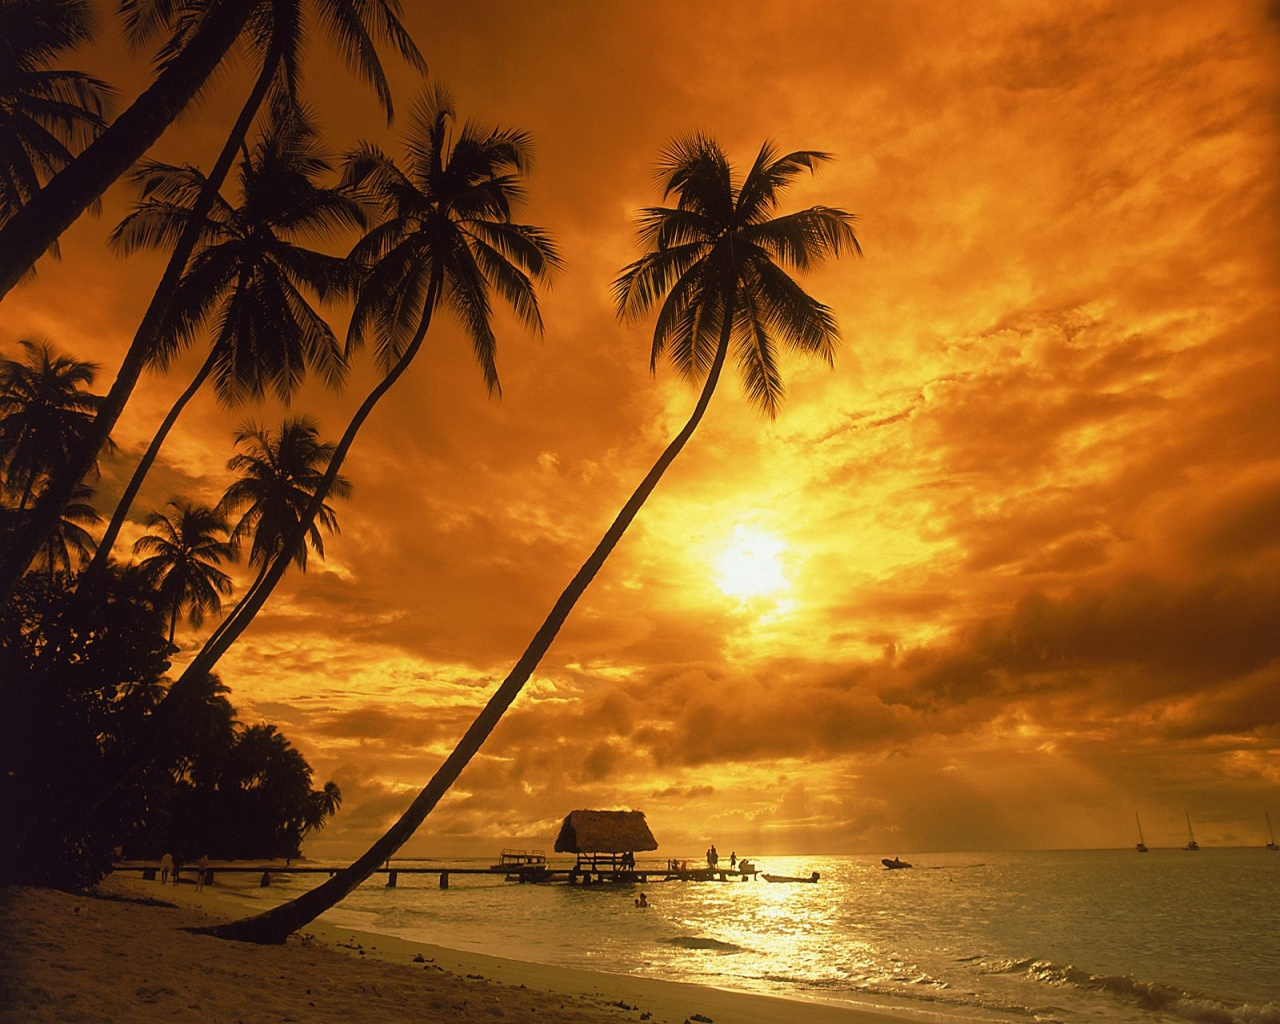
\includegraphics[width=0.8\textwidth]{pigeon_point_at_sunset-1280x1024.jpg} \\

}


\frame
{ \frametitle{What is that \texttt{command} column again?}
\begin{itemize}
 \item column ``command`` of type pg\_ddl\_command
 \item internal type, cannot be output directly
 \item pointer to a C struct
 \item can be passed to a C-language function for further processing
 \item \url{https://www.postgresql.org/message-id/20150409161419.GC4369@alvh.no-ip.org}
\end{itemize}

}

\begin{frame}[fragile]
\frametitle{\texttt{pg\_ddl\_command}}

\lstset{language=C}
\tiny
\begin{columns}

\begin{column}{0.5\textwidth}
\begin{lstlisting}
typedef struct CollectedCommand
{
    CollectedCommandType type;
    bool        in_extension;
    Node       *parsetree;

    union
    {
        /* most commands */
        struct
        {
            ObjectAddress address;
            ObjectAddress secondaryObject;
        } simple;

        /* GRANT / REVOKE */
        struct
        {
            InternalGrant *istmt;
        } grant;

        /* ALTER TABLE */
        struct
        {
            Oid    objectId;
            Oid    classId;
            List  *subcmds;
        } alterTable;


\end{lstlisting}
\end{column}

\begin{column}{0.5\textwidth}
\begin{lstlisting}
typedef enum CollectedCommandType
{
    SCT_Simple,
    SCT_AlterTable,
    SCT_Grant,
    SCT_AlterOpFamily,
    SCT_AlterDefaultPrivileges,
    SCT_CreateOpClass,
    SCT_AlterTSConfig
} CollectedCommandType;

typedef struct ObjectAddress
{
    Oid    classId;     /* Class Id from pg_class */
    Oid    objectId;    /* OID of the object */
    int32  objectSubId; /* Subitem within object */
} ObjectAddress;

typedef struct CollectedATSubcmd
{
    /* affected column, constraint, index, ... */
    ObjectAddress address;
    Node      *parsetree;
} CollectedATSubcmd;

\end{lstlisting}


\end{column}


\end{columns}
\end{frame}

\frame
{ \frametitle{The JSON output}

\begin{itemize}
\item We have an extension with a function that receives \texttt{pg\_ddl\_command} and returns JSON
\item In the event trigger function you can modify the JSON
\item We have a function to convert JSON back to text
\end{itemize}
}

\begin{frame}[fragile]
\frametitle{A JSON blob}
\lstset{language=json}
\scriptsize
\begin{lstlisting}
{   "fmt": "CREATE %{persistence}s TABLE %{identity}D
            %{if_not_exists}s (%{table_elements:, }s) 
            %{inherits}s %{on_commit}s %{tablespace}s", 
    "persistence": "UNLOGGED", 
    "identity": {
        "objname": "t1", 
        "schemaname": "public" }, 
    "if_not_exists": {
        "fmt": "IF NOT EXISTS",
        "present": false },
    "inherits": {
        "fmt": "INHERITS (%{parents:, }D)", 
        "parents": null, 
        "present": false }, 
    "on_commit": {
        "fmt": "ON COMMIT %{on_commit_value}s", 
        "on_commit_value": null, 
        "present": false }, 
    "table_kind": "plain",
    "tablespace": {
        "fmt": "TABLESPACE %{tablespace}I",
        "present": false,
        "tablespace": null }
}
\end{lstlisting}
\end{frame}

\begin{frame}[fragile]
\frametitle{A JSON blob (2)}
\lstset{language=json}
\scriptsize
\begin{lstlisting}
    "fmt": " ... (%{table_elements:, }s) ..."
    "table_elements": [
        {
            "fmt": "%{name}I %{coltype}T %{default}s
                    %{not_null}s %{collation}s", 
            "type": "column"
            "name": "a", 
            "not_null": "NOT NULL", 
            "collation": {
                "fmt": "COLLATE %{name}D", 
                "present": false
            }, 
            "coltype": {
                "is_array": false, 
                "schemaname": "pg_catalog", 
                "typename": "int4", 
                "typmod": ""
            }, 
            "default": {
                "default": "nextval('t1_a_seq'::regclass)", 
                "fmt": "DEFAULT %{default}s"
            }, 
        }
    ], 
\end{lstlisting}
\end{frame}

\frame
{ \frametitle{Possible ``fmt'' escapes}

\begin{description}
\item[\%\%] expand to a literal %.
\item[\%\{name\}I] expand as a single, non-qualified identifier
\item[\%\{name\}D] expand as a possibly-qualified identifier
\item[\%\{name\}T] expand as a type name
\item[\%\{name\}O] expand as an operator name
\item[\%\{name\}L] expand as a string literal (quote using single quotes)
\item[\%\{name\}s] expand as a simple string (no quoting)
\item[\%\{name\}n] expand as a simple number (no quoting)
\item[\%\{name\}R] expand as a role name (possibly quoted name, or PUBLIC)
\end{description}
}

\begin{frame}[fragile]
\frametitle{Helper functions}

\begin{itemize}
\item \texttt{pg\_event\_trigger\_expand\_command(jsonb)}
\end{itemize}

\begin{lstlisting}
CREATE UNLOGGED TABLE public.t1 
     (a pg_catalog.int4
      DEFAULT nextval('t1_a_seq'::regclass)
      NOT NULL )
\end{lstlisting}

\begin{itemize}
\item \texttt{jsonb\_set(json, path, value)}
\end{itemize}

\end{frame}

\frame
{ \frametitle{The AXLE project}

        Advanced Analytics for eXtremely Large European Databases \\

        \raggedleft
        {\LARGE \url{http://www.axleproject.eu/} }

    \vfill

\begin{columns}

\begin{column}{0.3\textwidth}
    \href{http://www.axleproject.eu/}{
\includegraphics{axle-logo-weights.jpg}}
\end{column}
\begin{column}{0.7\textwidth}
\raggedleft \footnotesize
The research leading to these results has received funding from the European Union's \href{http://ec.europa.eu/research/fp7/index_en.cfm}{\underline{Seventh Framework Programme (FP7/2007-2013)}} under grant agreement n° 318633
\end{column}
\end{columns}
}

\frame
{ \frametitle{Questions?}

\begin{itemize}
\item Thanks for listening
\item Please give feedback on the JSON side of things
\end{itemize}
}

\frame
{

\vfill

this page intentionally left blank

}

\frame
{ \frametitle{Event Triggers: Development History}

\begin{itemize}
\item
\textit{thread:} \href{http://example.com}{\texttt{[HACKERS] Command Triggers}} \\
135 messages, 10 patch versions: Nov 2011 -- Mar 2012 \\
{\tiny \url{http://www.postgresql.org/message-id/m2pqh2mrq6.fsf@2ndQuadrant.fr}}

\item 
\textit{thread:} \texttt{[HACKERS] Command Triggers, patch v11} \\
115 messages, 5 patch versions: Feb 2012 -- Mar 2012  \\
{\tiny \url{http://www.postgresql.org/message-id/m24nufq466.fsf@2ndQuadrant.fr}}

\item 
\textit{thread:} \texttt{[HACKERS] Command Triggers, v16} \\
 51 messages, 1 patch version: March 2012 \\
{\tiny \url{http://www.postgresql.org/message-id/m2r4wtohqn.fsf@2ndQuadrant.fr}}

\item 
\texttt{Subject: [HACKERS] Command Triggers (v17)} \\
1 message, 1 patch version: March 2012 \\
{\tiny \url{http://www.postgresql.org/message-id/m23995lerl.fsf@2ndQuadrant.fr}}

\item 
\textit{thread:} \texttt{[HACKERS] Command Triggers patch v18} \\
43 messages, 1 patch version: Mar 2012 -- Apr 2012 \\
{\tiny \url{http://www.postgresql.org/message-id/m2sjh35fj7.fsf@2ndQuadrant.fr}}
\end{itemize}

}

\frame
{ \frametitle{Event Triggers: Development History}
\begin{itemize}

\item 
\textit{thread:} \texttt{[HACKERS] Event Triggers reduced, v1} \\
64 messages, 10 patch versions: Jun 2012 -- Aug 2012 \\
{\tiny \url{http://www.postgresql.org/message-id/m2aa04jp6h.fsf@hi-media.com}}

\item \textit{commit:}
Syntax support and documentation for event triggers. \\
Date: Wed Jul 18 10:16:16 2012 -0400
%\item  56 files changed, 2398 insertions(+), 18 deletions(-)
{\tiny \url{http://git.postgresql.org/pg/commitdiff/3855968f328918b6cd1401dd11d109d471a54d40}}

\item \textit{commit:}
Make new event trigger facility actually do something. \\
Date: Fri Jul 20 11:38:47 2012 -0400
%\item  28 files changed, 1087 insertions(+), 197 deletions(-)
{\tiny \url{http://git.postgresql.org/pg/commitdiff/3a0e4d36ebd7f477822d5bae41ba121a40d22ccc}}

\end{itemize}
}

\frame
{ \frametitle{Event Triggers: Development History}
\begin{itemize}

\item 
\textit{thread:} \texttt{[HACKERS] Event Triggers: adding information} \\
114 messages, 9 patch versions: December 2012 \\
{\tiny \url{http://www.postgresql.org/message-id/m2txrsdzxa.fsf@2ndQuadrant.fr}}

\item \textit{commit:}
Add ddl\_command\_end support for event triggers. \\
Date: Mon Jan 21 18:00:24 2013 -0500
%\item  8 files changed, 390 insertions(+), 152 deletions(-)
{\tiny \url{http://git.postgresql.org/pg/commitdiff/841a5150c575ccd89e4b03aec66eeeefb21f3cbe}}

\end{itemize}
}

\frame
{ \frametitle{Event Triggers: Development History}
\begin{itemize}

\item 
\textit{thread:} \texttt{[HACKERS] sql\_drop Event Trigger} \\
94 messages, 13 patch versions: Jan 2013 -- Mar 2013 \\
{\tiny \url{http://www.postgresql.org/message-id/m2fw1ieq5x.fsf@2ndQuadrant.fr}}

\item \textit{commit:}
Allow extracting machine-readable object identity \\
Date: Wed Mar 20 18:19:19 2013 -0300
{\tiny \url{http://git.postgresql.org/pg/commitdiff/f8348ea32ec8d713cd6e5d5e16f15edef22c4d03}}

\item \textit{commit:}
Add sql\_drop event for event triggers \\
Date: Thu Mar 28 13:05:48 2013 -0300 \\
%\item  15 files changed, 1083 insertions(+), 115 deletions(-)
{\tiny \url{http://git.postgresql.org/pg/commitdiff/473ab40c8bb3fcb1a7645f6a7443a0424d70fbaf}}

\end{itemize}
}


\frame
{ \frametitle{Event Triggers: Development History}
\begin{itemize}

\item 
\textit{thread:} \texttt{[HACKERS] Add CREATE support to event triggers} \\
106 messages, 9 patch versions: Nov 2013 -- Jun 2014 \\
{\tiny \url{http://www.postgresql.org/message-id/20131108153322.GU5809@eldon.alvh.no-ip.org}}

\item 
\textit{thread:} \texttt{[HACKERS] deparsing utility commands} \\
54 messages, 12 patch versions: February 2015 -- May 2015 \\
{\tiny \url{http://www.postgresql.org/message-id/20150215044814.GL3391@alvh.no-ip.org}}

\item \textit{commit:}
Allow on-the-fly capture of DDL event details \\
Date: Mon May 11 19:14:31 2015 -0300 \\
% 72 files changed, 2667 insertions(+), 155 deletions(-)
{\tiny \url{http://git.postgresql.org/pg/commitdiff/b488c580aef4e05f39be5daaab6464da5b22a494}}

\end{itemize}
}

